\documentclass[11pt,]{article}
\usepackage{lmodern}
\usepackage{amssymb,amsmath}
\usepackage{ifxetex,ifluatex}
\usepackage{fixltx2e} % provides \textsubscript
\ifnum 0\ifxetex 1\fi\ifluatex 1\fi=0 % if pdftex
  \usepackage[T1]{fontenc}
  \usepackage[utf8]{inputenc}
\else % if luatex or xelatex
  \ifxetex
    \usepackage{mathspec}
  \else
    \usepackage{fontspec}
  \fi
  \defaultfontfeatures{Ligatures=TeX,Scale=MatchLowercase}
\fi
% use upquote if available, for straight quotes in verbatim environments
\IfFileExists{upquote.sty}{\usepackage{upquote}}{}
% use microtype if available
\IfFileExists{microtype.sty}{%
\usepackage{microtype}
\UseMicrotypeSet[protrusion]{basicmath} % disable protrusion for tt fonts
}{}
\usepackage[margin=1in]{geometry}
\usepackage[unicode=true]{hyperref}
\PassOptionsToPackage{usenames,dvipsnames}{color} % color is loaded by hyperref
\hypersetup{
            pdftitle={Project Proposal},
            colorlinks=true,
            linkcolor=Maroon,
            citecolor=blue,
            urlcolor=blue,
            breaklinks=true}
\urlstyle{same}  % don't use monospace font for urls
\usepackage{natbib}
\bibliographystyle{plainnat}
\usepackage{graphicx,grffile}
\makeatletter
\def\maxwidth{\ifdim\Gin@nat@width>\linewidth\linewidth\else\Gin@nat@width\fi}
\def\maxheight{\ifdim\Gin@nat@height>\textheight\textheight\else\Gin@nat@height\fi}
\makeatother
% Scale images if necessary, so that they will not overflow the page
% margins by default, and it is still possible to overwrite the defaults
% using explicit options in \includegraphics[width, height, ...]{}
\setkeys{Gin}{width=\maxwidth,height=\maxheight,keepaspectratio}
\setlength{\emergencystretch}{3em}  % prevent overfull lines
\providecommand{\tightlist}{%
  \setlength{\itemsep}{0pt}\setlength{\parskip}{0pt}}
\setcounter{secnumdepth}{0}
% Redefines (sub)paragraphs to behave more like sections
\ifx\paragraph\undefined\else
\let\oldparagraph\paragraph
\renewcommand{\paragraph}[1]{\oldparagraph{#1}\mbox{}}
\fi
\ifx\subparagraph\undefined\else
\let\oldsubparagraph\subparagraph
\renewcommand{\subparagraph}[1]{\oldsubparagraph{#1}\mbox{}}
\fi

% set default figure placement to htbp
\makeatletter
\def\fps@figure{htbp}
\makeatother



% Stuff I added.
% --------------

\usepackage{indentfirst}
\usepackage[doublespacing]{setspace}
\usepackage{fancyhdr}
\pagestyle{fancy}
\usepackage{layout}   
\lhead{\sc Project Proposal}
\chead{}
\rhead{\thepage}
\lfoot{}
\cfoot{}
\rfoot{}

\renewcommand{\headrulewidth}{0.0pt}
\renewcommand{\footrulewidth}{0.0pt}

\usepackage{sectsty}
\sectionfont{\centering}
\subsectionfont{\centering}

\newtheorem{hypothesis}{Hypothesis}

% Begin document
% --------------

\begin{document}

\doublespacing

\begin{titlepage}
    \begin{center}
    \line(1,0){300} \\ 
    [0.25in]
    \huge{\bfseries Project Proposal} \\
    [2mm]
    \line(1,0){200} \\
    [1.5cm] 
    \textsc{\Large Key Reinstallation Attacks on Wi-Fi Networks} \\
    [0.75cm]
    \textsc{\Large Mobile Application to raise awareness} \\
    [10cm]
    \end{center}
    
    \begin{flushright}
    \textsc{\Large{Gurpreet S, Konrad P, Logan K, Fernando C \\} \normalsize\emph{Software Developers \\} }
    
    \end{flushright}
    
\end{titlepage}

\newpage

{
\hypersetup{linkcolor=black}
\setcounter{tocdepth}{2}
\tableofcontents
\newpage
}


\begin{center}\textbf{Abstract}\end{center}

\noindent Bringing awareness to new attacks that expose the majority of WiFi
networks. This proposal discusses the importance of recent attacks
executed on the WPA2 protocol and proposes the creation of a mobile
application that can showcase and exploit wireless APs.




\section{Attack Description}\label{attack-description}

Since it's introduction in 2006, WPA2 has become the most popular
protected access technology used in the consumer industry. Almost every
household WiFi network is currently making use of WPA2 to authenticate
its devices.

On October 16th, 2017 a flaw was found in the WPA2 protocol, making
every device using it to connect to a Wi-Fi network vulnerable and
helpless to hackers. No matter the encryption method, from WPA2 to AES,
hackers are able to decrypt any data sent by the victim. In fact,
because this is a man in the middle attack, the device can be tricked
into using an all-zero encryption key. If no other form of encryption is
utilized (HTTPS), the attacker will have access to unencrypted and
human-readable data, even when it comes to sensitive information like
usernames, passwords, and credit-card information. If that isn't bad
enough, it is even possible to inject ransomware or malware into
websites. Meaning, this is not only bad for the users but also the web
providers. The worst part is that there is no way to stop this, other
than hardwiring the device, or hoping the manufacturer of the device
offers an update that patches this attack. \citet{KrackAttacks}

The method of using this weakness in Wi-Fi is called a Key
Reinstallation Attack (KRACK). Every modern Wi-Fi standard uses a 4-way
handshake to connect. This is where the server and client agree on an
encryption key to use when encrypting and decrypting all future
messages. The attack occurs in the third message of the 4-way handshake.
What happens is the hacker tricks the victim into reinstalling the
encryption key that is already in use. This is achieved through
manipulation and replaying of cryptographic handshake messages.
Theoretically, it should not be possible to install the same key
multiple times in a row, but because it is very common for messages sent
over Wi-Fi to get lost, many messages in this handshake may need to be
retransmitted. This makes the attack able to reset the nonce any time it
retransmits this third message, enabling packets to be replayed, then
decrypted and even forged. The whole purpose of this nonce was to ensure
that past massages could not be reused in replay attacks.

There are many variations of this attack that have been discovered that
have varying levels of impact. One of the worst and most devastating is
being able to reinstall an all-zero encryption key. Being the worst
variation one would hope it is not too common, however, all devices
using Linux or Android 6+ are susceptible. This all-zero encryption key
makes it easy to manipulate and intercept data sent at will since all of
this data is now readable text. With so many Linux and Android devices
present, this is especially scary and concerning. Even more so with
their only hope being to wait for a security update to fix this
vulnerability.

\section{The Goal}\label{the-goal}

With this project we are trying to educate average Wi-Fi users and show
them the power of this exploit. The only way to eliminate this attack
vector is to patch every access point. If consumers are not concerned
with this attack manufacturers are not going to be motivated to produce
a patch for their devices. Therefore, we are hoping that consumers see
the effects of a key reinstallation attack and show manufacturers that
they need an update. By raising awareness the ultimate goal of secure
Wi-Fi can be achieved.

\section{Proposed Solution}\label{proposed-solution}

\subsection{Description}\label{description}

Our proposed solution is to create a mobile application on both iOS and
Android showcasing the attack's capabilities. Not only will the bring
awareness to the issue, but will let users actually test to see if any
of their personal devices are prone to this attack. Furthermore, it will
actually allow the user to perform the task and see the decrypted data
to allow them to truly understand the dangers. The application will have
3 screens. The first one describing the functionality as well a warning
informing the user to only use the app on APs they own. The second
screen will allow searching nearby APs and provide a list to choose
from. Once the user selects an access point from the list, they will be
shown details about the device and buttons for initializing the attack
and collecting data.

\subsection{Competition}\label{competition}

Since this is such a new exploit there are no other competitors
attempting to do the same thing. Only resources available are the
official technical demonstrations and paper created by the researchers
that discovered this attack. We hope to be the first ones to provide an
application like around this research.

\subsection{Project Milestones}\label{project-milestones}

The development structure for this application will start with a series
of proof of concepts (POC) following the technical description of the
attack. Then the working POCs will be integrated into a mobile
application

\begin{figure}
\centering
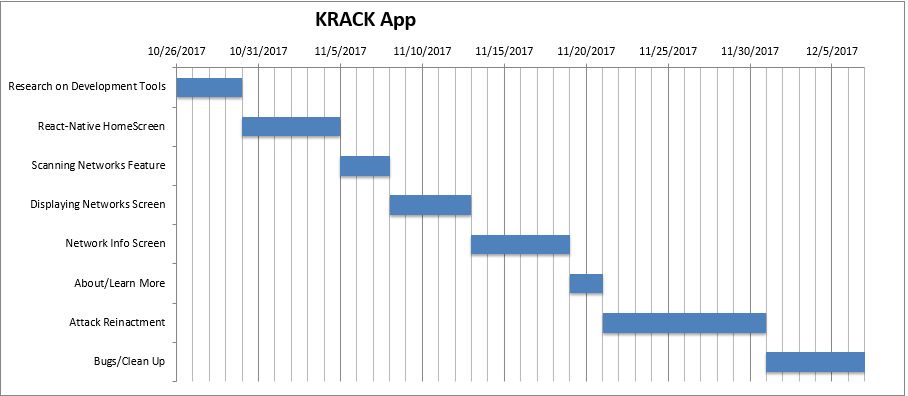
\includegraphics{images/gantt.png}
\caption{Gantt}
\end{figure}

\newpage

\section{App Mockups}\label{app-mockups}

\begin{figure}
\centering
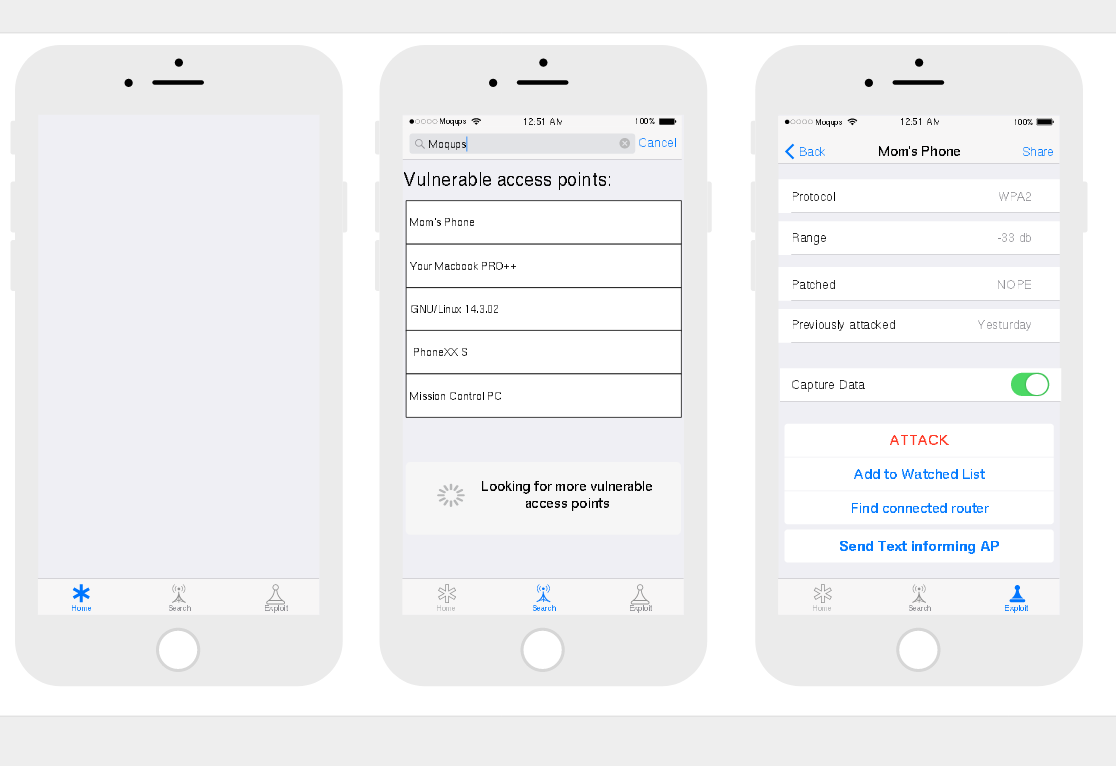
\includegraphics{images/mockup.png}
\caption{Mockups}
\end{figure}

\newpage

\bibliography{bibliography.bib}

\end{document}

